\documentclass[a4paper, 12pt]{article}
\usepackage{tikz}
\usetikzlibrary{shapes,arrows}
\usepackage[portuguese]{babel}
\usepackage[utf8]{inputenc}
\usepackage{amsmath}
\usepackage{enumerate}
\usepackage[pdftex]{hyperref}
\usepackage{graphicx}
\usepackage{placeins}
\tikzstyle{decision} = [diamond, draw, fill=blue!20, 
    text width=4.5em, text badly centered, node distance=3cm, inner sep=0pt]
\tikzstyle{block} = [rectangle, draw, fill=blue!20, 
    text width=8em, text centered, rounded corners, minimum height=4em]
\tikzstyle{line} = [draw, -latex']
\hypersetup{
  colorlinks,
  citecolor=blue,
  filecolor=blue,
  linkcolor=red,
}
\title{UFSC / CTC / INE \\
{\bf Disciplina: Redes de Computadores} \\
{\bf Trabalho Prático 2}}

\author{ {\bf Curso de Sistemas de Informação: INE5615-05238}  \\
  Vitor Arins  \\
  Matrícula: 12205530
}

\date{\today}
\begin{document}
\maketitle

\FloatBarrier
\paragraph{\underline{Respostas Parte 1}}

\begin{enumerate}
  \setcounter{enumi}{6}

\FloatBarrier
\item Print do comando {\bf ifconfig}:

\begin{figure}[h!]
\centering
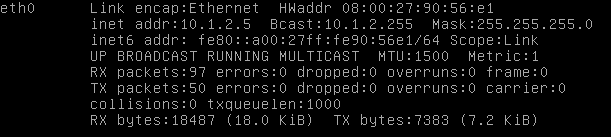
\includegraphics[width=\textwidth]{1-ifconfig-dream.png}
\caption{ifconfig dream}
\end{figure}

\begin{figure}[h!]
\centering
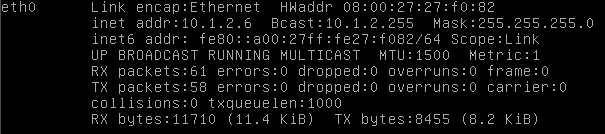
\includegraphics[width=\textwidth]{1-ifconfig-lucien.png}
\caption{ifconfig lucien}
\end{figure}

\begin{figure}[h!]
\centering
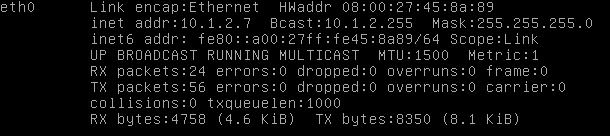
\includegraphics[width=\textwidth]{1-ifconfig-barnabas.png}
\caption{ifconfig barnabas}
\end{figure}

\FloatBarrier
\item Print dos comandos {\bf ping}:

\begin{figure}[h!]
\centering
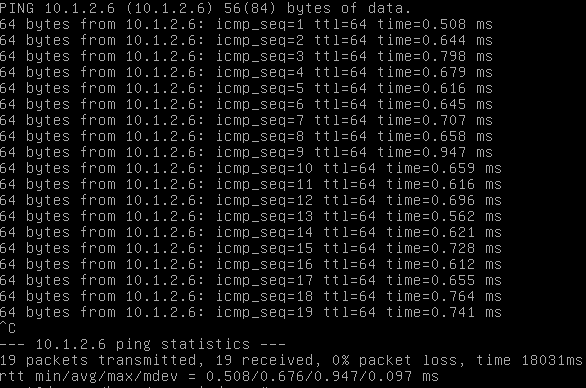
\includegraphics[width=\textwidth]{1-ping-dream-lucien.png}
\caption{{\bf ping} da máquina {\bf dream} para máquina {\bf lucien}}
\end{figure}

\begin{figure}[h!]
\centering
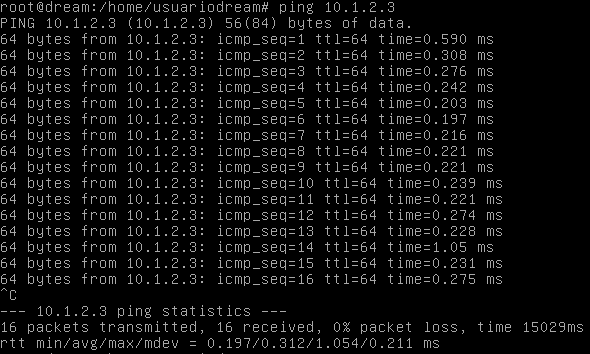
\includegraphics[width=\textwidth]{1-ping-dream-VB.png}
\caption{{\bf ping} da máquina {\bf dream} para conexão {\bf VirtualBox}}
\end{figure}

\begin{figure}[h!]
\centering
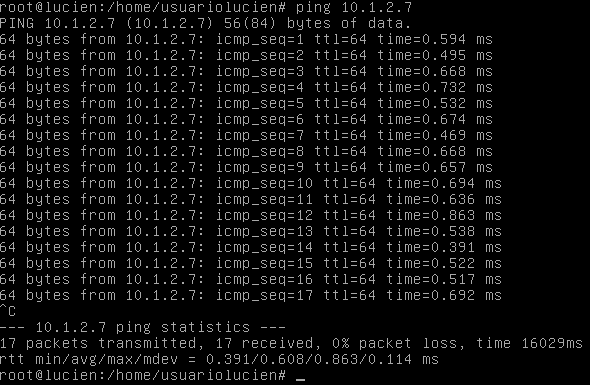
\includegraphics[width=\textwidth]{1-ping-lucien-barnabas.png}
\caption{{\bf ping} da máquina {\bf lucien} para máquina {\bf barnabas}}
\end{figure}

\begin{figure}[h!]
\centering
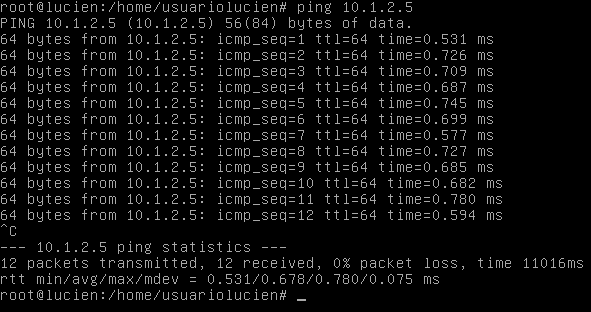
\includegraphics[width=\textwidth]{1-ping-lucien-dream.png}
\caption{{\bf ping} da máquina {\bf lucien} para máquina {\bf dream}}
\end{figure}

\begin{figure}[h!]
\centering
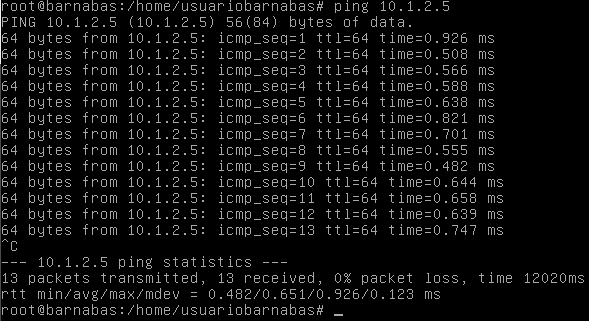
\includegraphics[width=\textwidth]{1-ping-barnabas-dream.png}
\caption{{\bf ping} da máquina {\bf barnabas} para máquina {\bf dream}}
\end{figure}

\begin{figure}[h!]
\centering
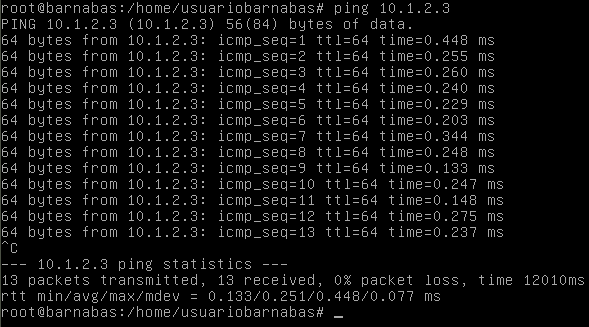
\includegraphics[width=\textwidth]{1-ping-barnabas-VB.png}
\caption{{\bf ping} da máquina {\bf barnabas} para conexão {\bf VirtualBox}}
\end{figure}

\FloatBarrier
\item A máquina {\bf lucien} não conseguiu ``pingar'' a máquina {\bf
    dream} pois após alterado o seu ip estava fora da faixa de ips
  conhecidos pelo DHCP.

\begin{figure}[h!]
\centering
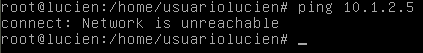
\includegraphics[width=\textwidth]{1-falha-ping-lucien-dream.png}
\caption{Falha do {\bf ping} da máquina {\bf lucien} para máquina {\bf dream}}
\end{figure}

\FloatBarrier
\item
\begin{enumerate}[a.]

\item Foi desativada a interface ``eth0'' e portanto a máquina perdeu
  conexão com a rede.

\FloatBarrier
\item Resultado:
\begin{figure}[h!]
\centering
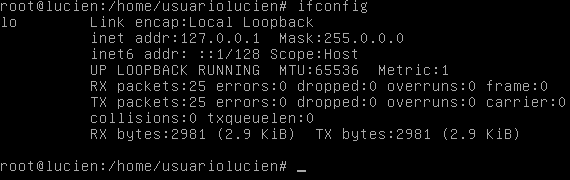
\includegraphics[width=\textwidth]{1-ifconfig-lucien-lo.png}
\caption{{\bf ifconfig} da máquina {\bf lucien} apenas com interface
  ``lo'' (loopback)}
\end{figure}

\item Foi restaurada a interface ``eth0'' e portanto a máquina
  recuperou sua conexão com a rede.

\FloatBarrier
\item Resultado:
\begin{figure}[h!]
\centering
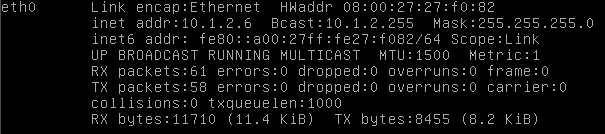
\includegraphics[width=\textwidth]{1-ifconfig-lucien.png}
\caption{{\bf ifconfig} da máquina {\bf lucien}}
\end{figure}

\item Foi possível \emph{pingar} a máquina {\bf dream} pois após
  reiniciar a interface de rede ``eth0'', a máquina {\bf lucien}
  recuperou seu IP antigo na faixa de endereços conhecidos pelo DHCP.

\end{enumerate}

\item 
\begin{enumerate}[a.]

\item Os endereços são da classe {\bf A}.

\item A máscara utilizada é a default: {\bf 255.255.255.0} ou {\bf /8}

\item O endereço de broadcast para a sub-rede é {\bf 10.1.2.255}

\end{enumerate}

\end{enumerate}

\FloatBarrier
\paragraph{\underline{Respostas Parte 2}}

\begin{enumerate}
  \setcounter{enumi}{5}

\item 
\begin{itemize}

  \item{e.} Foi possível pingar o host pois a máquina dream tem uma interface
    de rede ligada a rede da máquina hospedeira física que possui rota para o
    host www.inf.ufsc.br.
  \item{f.} Não é possível pingar o host pois não há rota que leve até
    o host 150.162.60.21.
  \item{g.} ``ping'' significa latência, serve para enviar pacotes e
    receber as respostas de um host em questão. A saída do comando
    ping mostra o tamanho do pacote enviado, a quantidade de pacotes
    enviadas ao host, o tempo de latência entre a máquina e o host e a
    quantidade de pacotes perdidos durante a operação.

\end{itemize}

\item
\begin{enumerate}

\item Significa que a máquina poderá visualizar a rota para a rede
  externa e ficará visível para a rede com o ip definido.

\item Agora é possível pingar o host 150.162.60.2 e enviar pacotes
  recebendo respostas.

\end{enumerate}

\item
\begin{enumerate}

\item O comando {\bf modprobe} carrega o módulo NAT. O comando {\bf
    iptables} adiciona (-A) regra (POSTROUTING) a tabela nat (-t nat)
  da fonte (-s 192.168.20.0/24) na interface de rede (-o eth0) com a
  ação MASQUERADE (mascaramento). Isso faz com que os pacotes oriundos
  da sub-rede possam ser redirecionados pela interface {\bf eth0} para
  a rede externa e vice-versa.

\item Foi possível pingar o host 150.162.2.10 enviando pacotes e
  recebendo as respostas.

\item Foi reescrito o arquivo /etc/resolv.conf

\item Não foi possível pingar o host www.ufsc.br pois o nome do host
  não foi resolvido.

\end{enumerate}

\item 
\begin{enumerate}

\item Foi possível pingar o host www.inf.ufsc.br, resolvendo-o para o
  ip 150.162.60.21 e enviando pacotes.

\end{enumerate}

\stepcounter{enumi}

\item Foi utilizada a sub-rede 172.16.40.0/8

\item Foram adicionadas regras para bloquear o acesso das máquinas
  {\bf lucien} e {\bf dream} para o site {\bf
    www.facebook.com}. 

\end{enumerate}

\end{document}